\documentclass{article}
% We will use NIPS submission format
\usepackage{nips13submit_e,times}
% for hyperlinks
\usepackage{hyperref}
\usepackage{url}
% For figures
\usepackage{graphicx}
\usepackage{subfigure}
% math packages
\usepackage{amsmath}
\usepackage{amsfonts}
\usepackage{amsopn}
\usepackage{ifthen}
\usepackage{natbib}

\title{Machine Learning Project II by Group KATHMANDU}

\author{
  Jade Copet\\
  EPFL \\
  \texttt{jade.copet@epfl.com} \\
  \And
  Merlin Nimier David\\
  EPFL \\
  \texttt{merlin.nimier-david@epfl.com} \\
  \And
  Krishna Raj Sapkota\\
  EPFL \\
  \texttt{krishna.sapkota@epfl.com} \\
}

\nipsfinalcopy

\begin{document}
\maketitle



\begin{abstract}
\end{abstract}



\section{Song recommendation}

  \subsection{Dataset description}
  \textbf{Objective}: The song recommendation dataset represents the musical habits of users on a musical streaming service. We are given a large number of (user, artist, listening count) triplets, as well as a friendship graph encoding the connections between users. Our goal is to use this training data to perform:

  \begin{itemize}
    \item \textit{Weak} generalization: for existing users, predict the listening counts for unobserved (user, artist) pairs.
    \item \textit{Strong} generalization: for unknown users, predict the listening counts. We may use the friendship data.
  \end{itemize}

  \textbf{About the data}: The listening counts matrix $Y$ covers $1774$ users and $15085$ artists. It is very sparse, as we observe only $69617$ triplets (density of $0.2\%$). The friendship graph $G$ is given in the form of a symmetric $1774 \times 1774$ adjacency matrix, where $G_{i, j} = G_{j, i} = 1$ if users $i$ and $j$ are connected.\\

  Artists have listening counts ranging from $1$ to $2274039$, the most listened artist being Britney Spears (for some reason). Over all observations, before any outlier removal, the average count is 707 while the median count is 278.\\

  TODO: explain carefully how we handled unobserved data.

  \textbf{Error measure}: Both weak and strong prediction involve generating, for all users, predicted listening counts for all artists. Each output is thus $15085$-dimensional. We use mean \textbf{RMSE} as our main error measure. Given a predicted matrix $\hat{Y}$, we first compute the RMSE for each artist, and then take the mean over all artists.\\
  TODO: is this the correct approach?

  \subsection{Dataset analysis and preprocessing}
  Examining the dataset, we noticed that user $385$ had listened to artist $9162$ a whopping $352698$ times. Assuming an average song duration of $3$ minutes, user $385$ have supposedly spent the equivalent of two full years listening to \textit{Depeche Mode}. It was then necessary to remove such outliers before carrying out any learning.

  Several Machine Learning techniques rely on the assumption that data follows a Gaussian distribution. Since observed listening counts are strictly positive, we normalized and centered the data. We assumed that it was important to take into account artist popularity, but not the volume of music consumption of users. Therefore, we normalized the counts so as to obtain comparable values among users, but retain difference of popularity between artists.

  \begin{figure}[ht]
    \center
    \subfigure{
      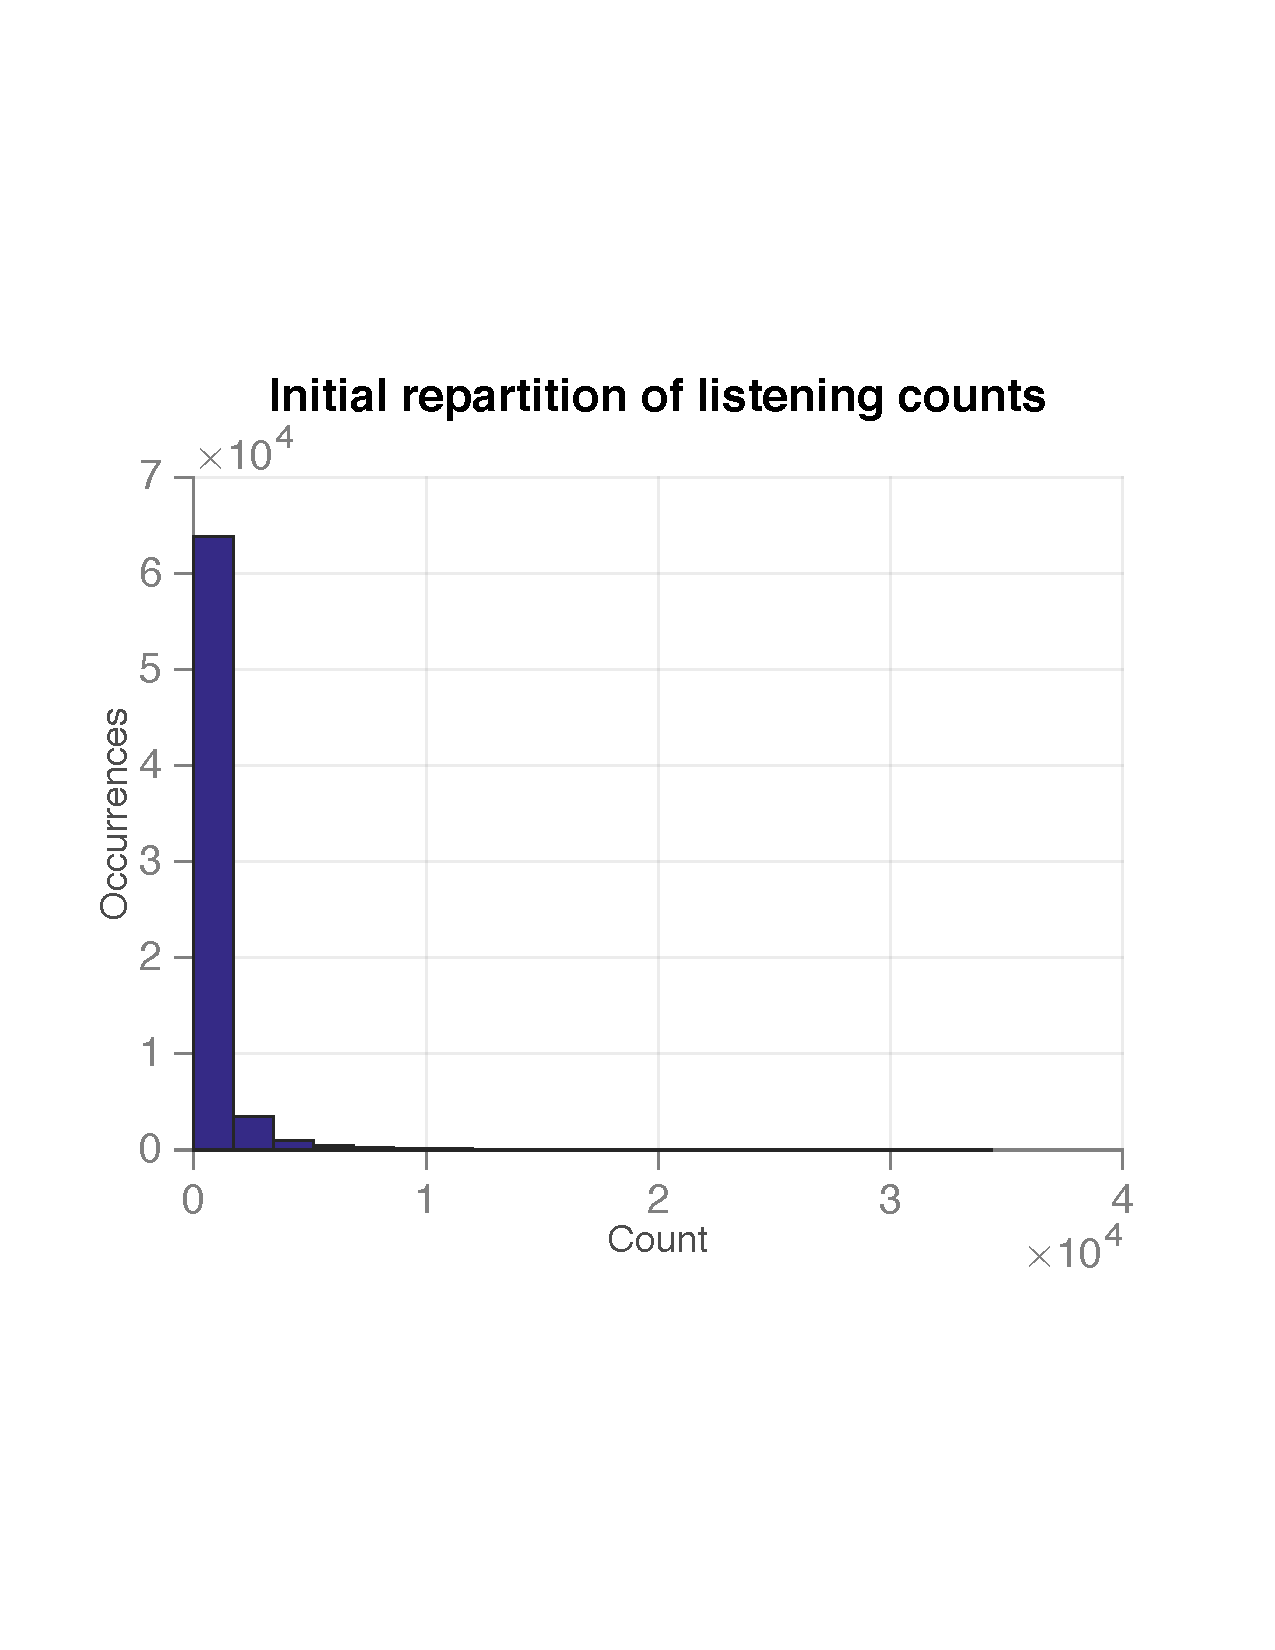
\includegraphics[width=2.5in]{figures/recommendation/unnormalized-counts.pdf}
    }
    \subfigure{
      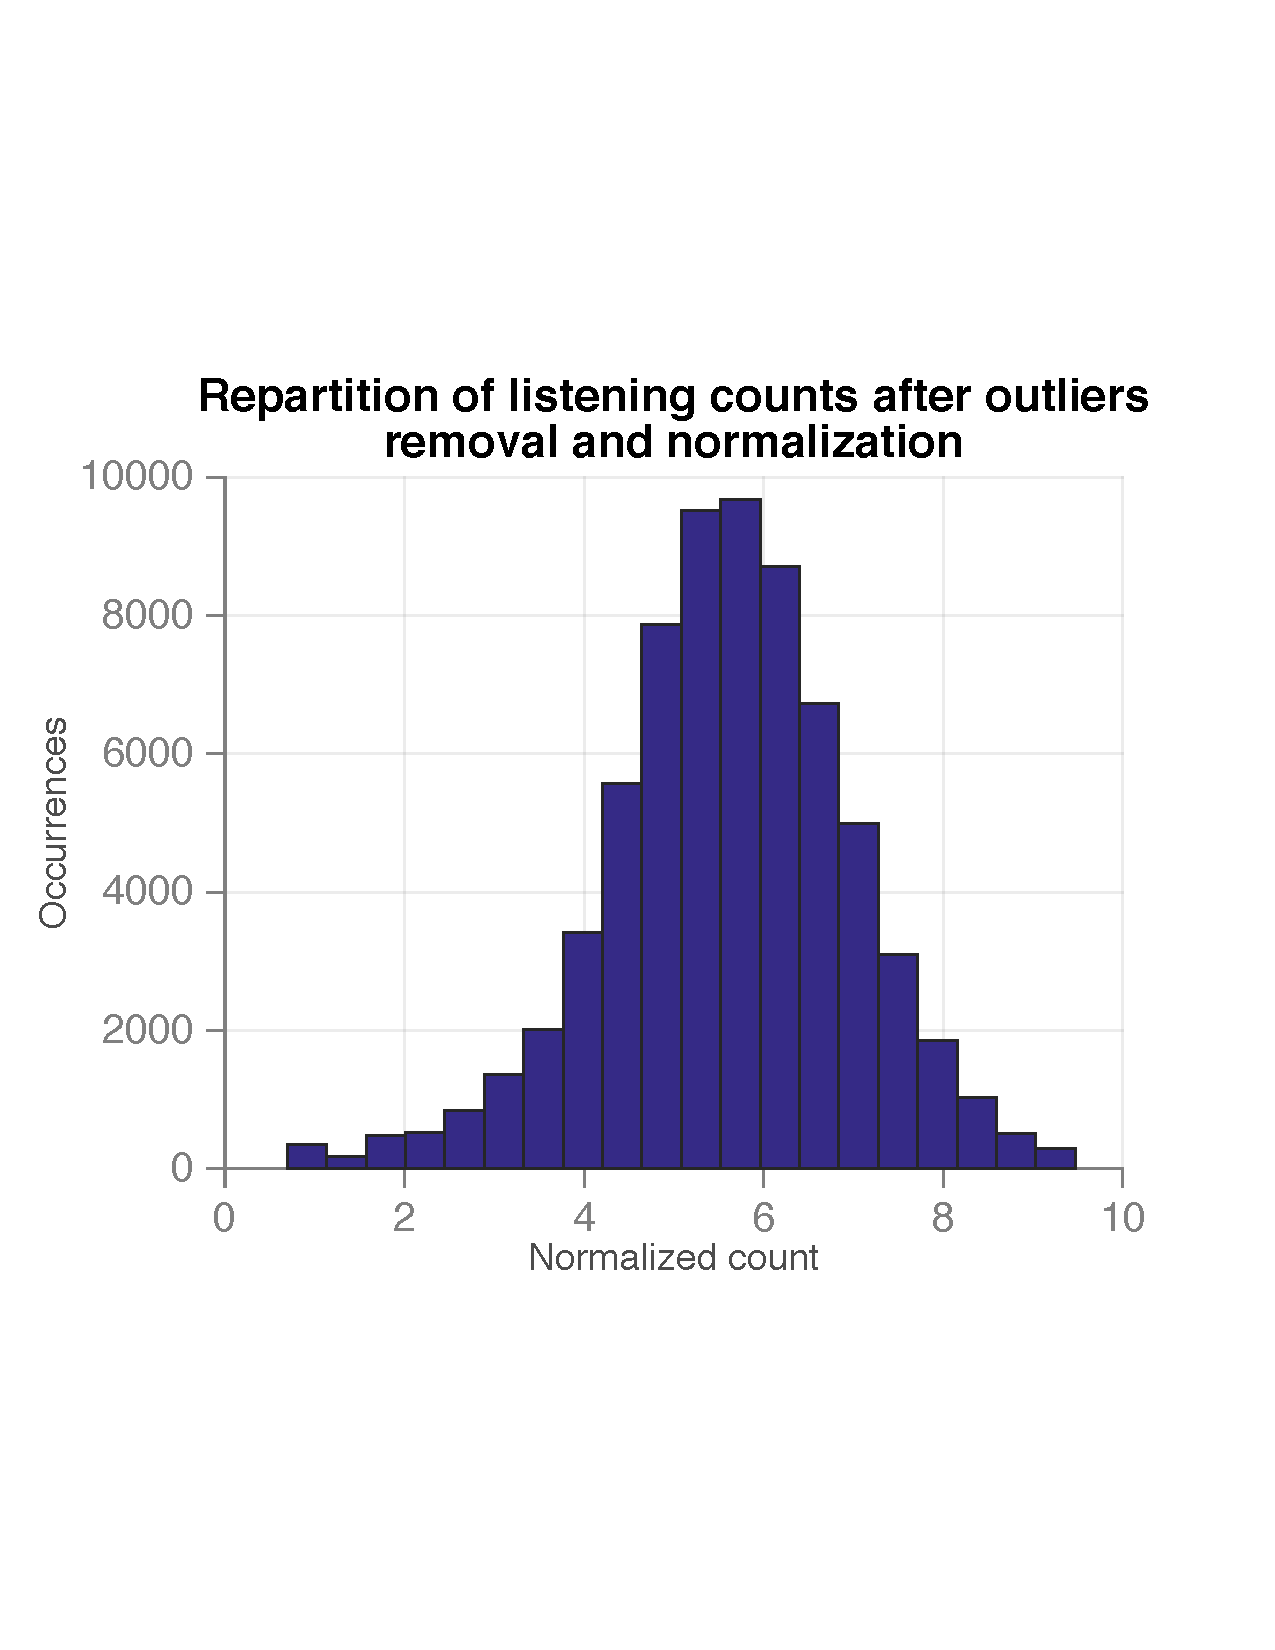
\includegraphics[width=2.5in]{figures/recommendation/normalized-counts.pdf}
    }
    \caption{Normalization makes listening counts distribution more Gaussian}
    \label{fig:recommendation-normalization}
  \end{figure}

  Finally, in order to test our models for both weak and strong predictions, we separated the training set in two ways:
  \begin{itemize}
    \item Entirely remove a proportion of users to use them as a strong prediction test set
    \item Withhold a proportion of the remaining (user, artist, listening count) triplets to use them as a weak prediction test set
  \end{itemize}

  \subsection{Feature transformations}

  \subsection{Final model and predictions}



\section{Image classification}

  \subsection{Dataset description}
  Task description

  Dataset characteristics. Features where provided (Piotr's toolbox).

  \subsection{Error measures}

  \subsection{Data visualization and cleaning}

  \subsection{Feature transformations}
  
   \subsection{Model selection}

  \subsection{Final model and predictions}



\section{Summary}
  Sparse matrix representation made manipulation less straightforward and required us to learn a few new techniques.

  \subsubsection*{Acknowledgments}

  \subsubsection*{References}

\end{document}
